%-------------------------------------------------------------------------------
% seq24_menu
%-------------------------------------------------------------------------------
%
% \file        seq24_menu.tex
% \library     Documents
% \author      Chris Ahlstrom
% \date        2015-07-19
% \update      2015-07-19
% \version     $Revision$
% \license     $XPC_GPL_LICENSE$
%
%     Provides the Menu section of seq24-user-manual.tex.
%
%-------------------------------------------------------------------------------

\section{Menu}
\label{sec:seq24_menu}

   The \textsl{Seq24} menu, as seen at the top of
   \figureref{fig:seq24_main_screen},
   is fairly simple, but it is important to understand the
   structure of the menu entries.

\subsection{Menu / File}
\label{subsec:seq24_menu_file}

   The \textbf{File} menu is used to save and load standard 
   MIDI files.  It should be able to handle any 
   Format 1 standard files that any other sequencer 
   is capable of exporting.  

   The \textsl{Seq24}
   menu entry contains the sub-items shown in
   \figureref{fig:seq24_menu_file_items}.
   The next few sub-sections discuss the sub-items in the 
   \textsl{File} sub-menu.

\begin{figure}[H]
   \centering 
   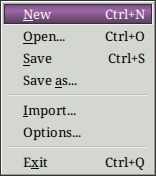
\includegraphics[scale=1.0]{menu/menu_file.png}
   \caption{Seq24 File Menu Items}
   \label{fig:seq24_menu_file_items}
\end{figure}

\subsection{Menu / File / New}
\label{subsec:menu_file_new}

   TODO

\subsubsection{Menu / File / Open}
\label{subsubsec:seq24_menu_file_open}

   TODO

\begin{figure}[H]
   \centering 
   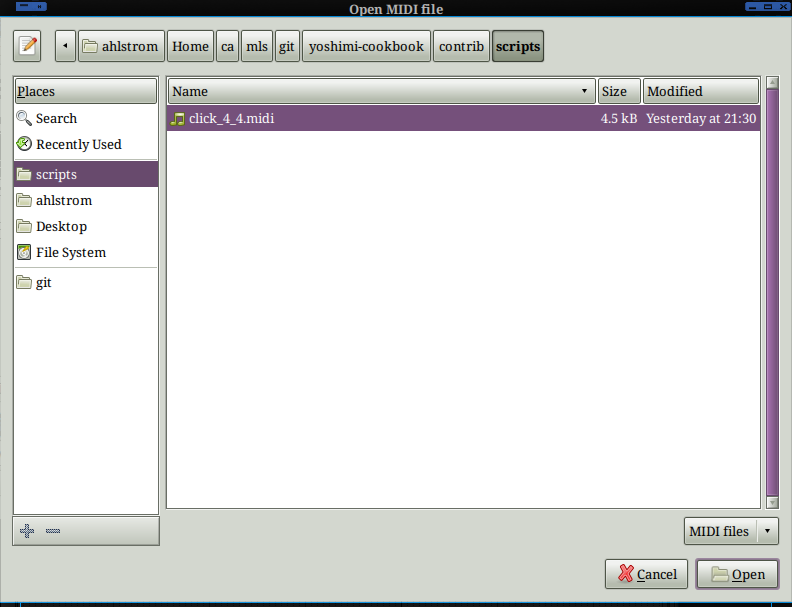
\includegraphics[scale=0.75]{menu/menu_file_open.png}
   \caption{File Open}
   \label{fig:seq24_menu_file_open}
\end{figure}

\subsubsection{Menu / File / Save (As)}
\label{subsubsec:menu_file_open_save_as}

   TODO

\begin{figure}[H]
   \centering 
   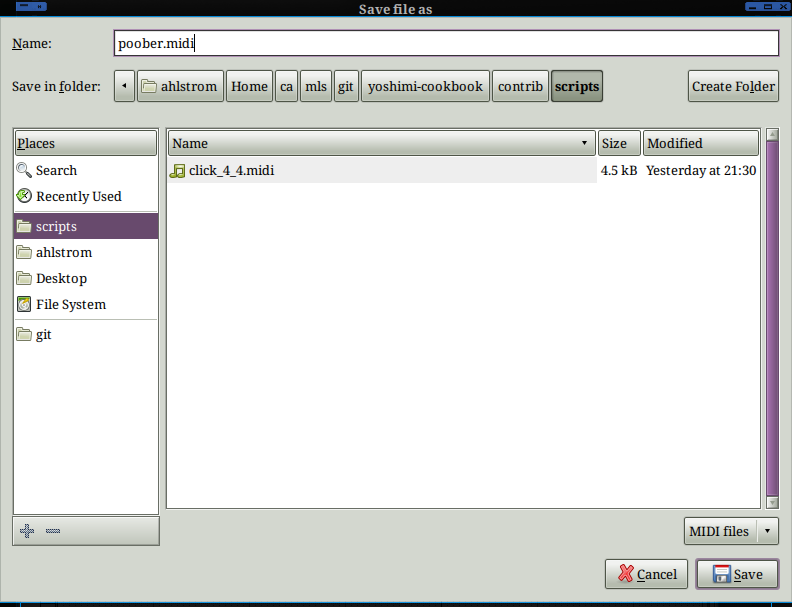
\includegraphics[scale=0.75]{menu/menu_file_save_as.png}
   \caption{File Save As}
   \label{fig:seq24_menu_file_save_as}
\end{figure}

   TODO

\subsubsection{Menu / File / Import}
\label{subsubsec:seq24_menu_file_import}

   TODO

\begin{figure}[H]
   \centering 
   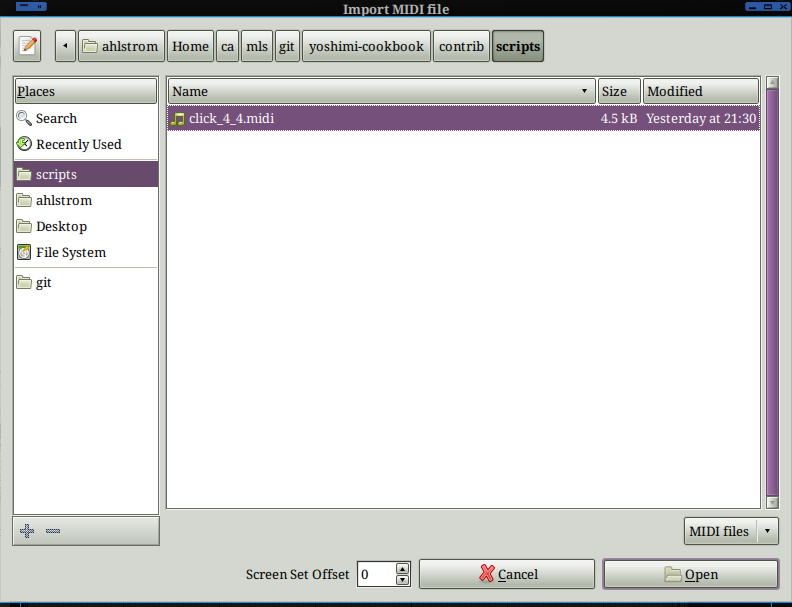
\includegraphics[scale=0.75]{menu/menu_file_import.png}
   \caption{File Import}
   \label{fig:seq24_menu_file_import}
\end{figure}

   TODO

\subsubsection{Menu / File / Options}
\label{subsubsec:seq24_menu_file_options}

   TODO

\paragraph{Menu / File / Options / MIDI Clock}
\label{paragraph:seq24_menu_file_options_midi_clock}

   TODO

\begin{figure}[H]
   \centering 
   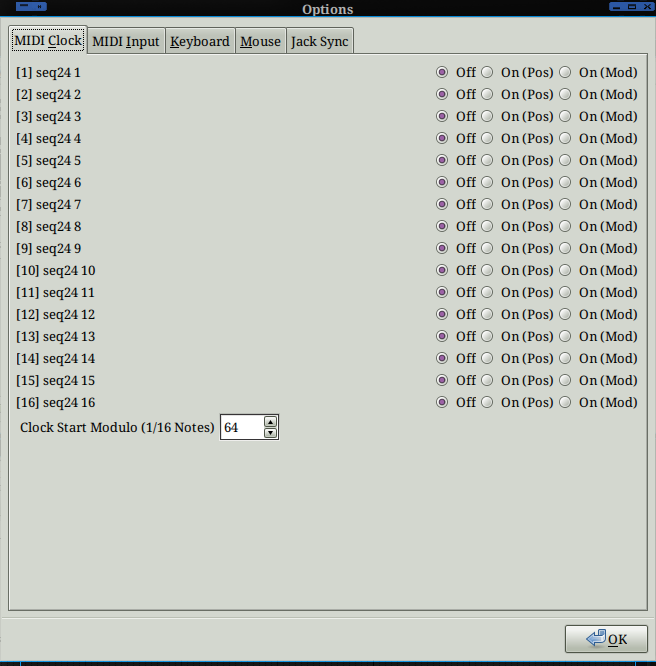
\includegraphics[scale=0.75]{menu/menu_file_options_midi_clock.png}
   \caption{File Options MIDI Clock}
   \label{fig:seq24_menu_file_options_midi_clock}
\end{figure}

   Used to configure to what bus the MIDI clock gets dumped.

\paragraph{Menu / File / Options / MIDI Input}
\label{paragraph:seq24_menu_file_options_midi_input}

   TODO

\begin{figure}[H]
   \centering 
   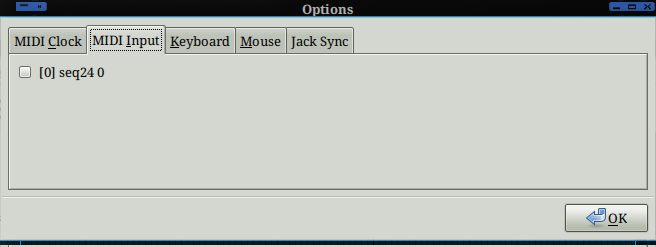
\includegraphics[scale=0.75]{menu/menu_file_options_midi_input_condensed.png}
   \caption{File Options MIDI Input (Condensed View)}
   \label{fig:seq24_menu_file_options_midi_input}
\end{figure}

   TODO

\paragraph{Menu / File / Options / Keyboard }
\label{paragraph:seq24_menu_file_options_keyboard}

   TODO

\begin{figure}[H]
   \centering 
   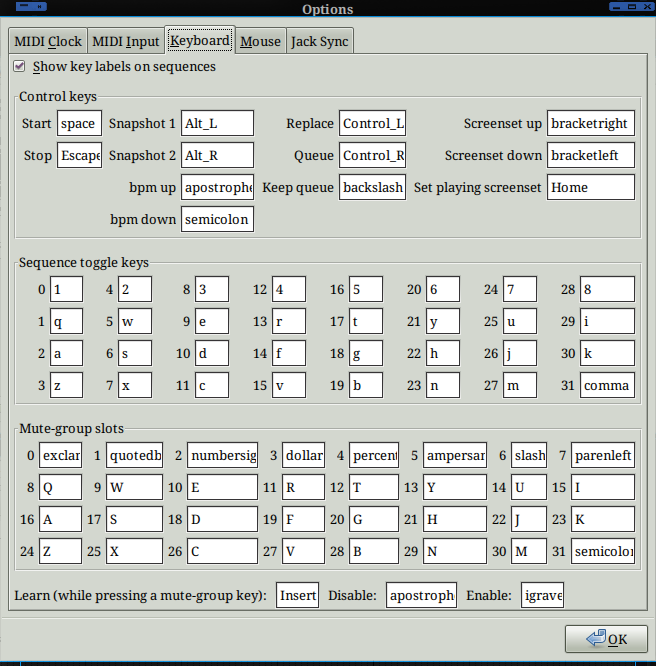
\includegraphics[scale=0.75]{menu/menu_file_options_keyboard.png}
   \caption{File Options Keyboard}
   \label{fig:seq24_menu_file_options_keyboard}
\end{figure}

   TODO

\paragraph{Menu / File / Options / Mouse }
\label{paragraph:seq24_menu_file_options_mouse}

   TODO

\begin{figure}[H]
   \centering 
   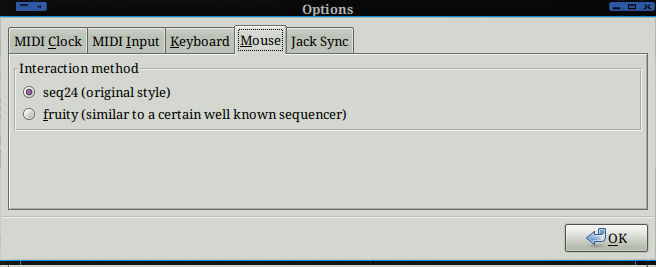
\includegraphics[scale=0.75]{menu/menu_file_options_mouse_condensed.png}
   \caption{File Options Mouse (Condensed View)}
   \label{fig:seq24_menu_file_options_mouse}
\end{figure}

   TODO

\paragraph{Menu / File / Options / Jack Sync }
\label{paragraph:seq24_menu_file_options_jack_sync}

   TODO

\begin{figure}[H]
   \centering 
   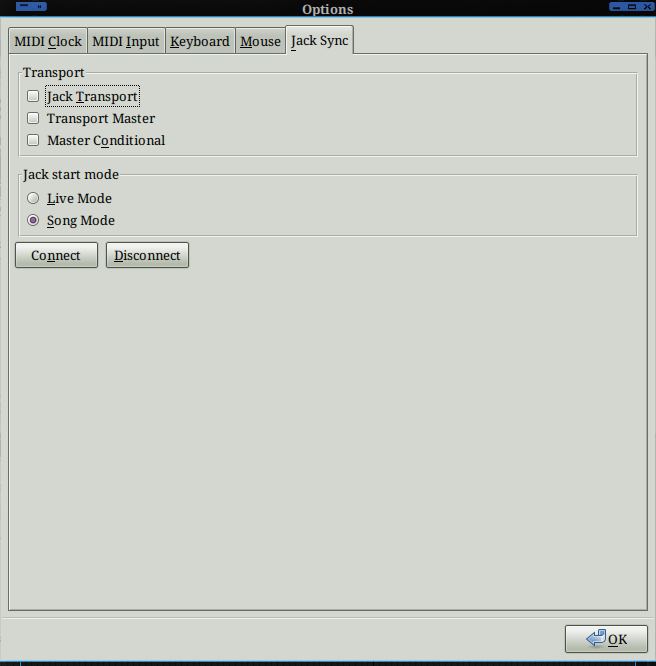
\includegraphics[scale=0.75]{menu/menu_file_options_jack_sync.png}
   \caption{File Options Jack Sync}
   \label{fig:seq24_menu_file_options_jack_sync}
\end{figure}

   TODO

\subsection{Menu / View}
\label{subsec:seq24_menu_view}

   TODO

\subsection{Menu / Help About...}
\label{subsec:seq24_menu_about}

   This menu entry shows the "About" dialog.

\begin{figure}[H]
   \centering 
   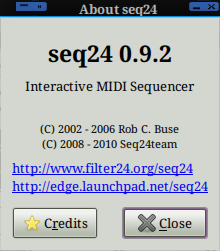
\includegraphics[scale=0.75]{menu/menu_help_about.png}
   \caption{Help About}
   \label{fig:seq24_menu_help_about}
\end{figure}

   That dialog provides access to the credits for the program, including the
   authors and the project documentor.

\begin{figure}[H]
   \centering 
   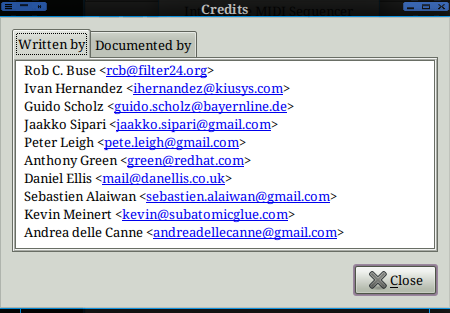
\includegraphics[scale=0.75]{menu/menu_help_credits.png}
   \caption{Help Credits}
   \label{fig:seq24_menu_help_credits}
\end{figure}

   TODO

\begin{figure}[H]
   \centering 
   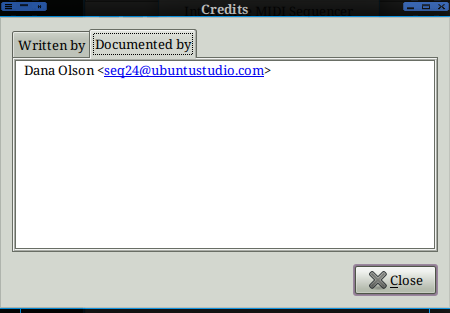
\includegraphics[scale=0.75]{menu/menu_help_doc.png}
   \caption{Help Documentation}
   \label{fig:seq24_menu_help_doc}
\end{figure}

   TODO


%-------------------------------------------------------------------------------
% vim: ts=3 sw=3 et ft=tex
%-------------------------------------------------------------------------------
